\documentclass[12pt,a4paper]{article}
\usepackage{amsmath,amscd,amsbsy,amssymb,latexsym,url,bm,amsthm}
\usepackage{epsfig,graphicx,subfigure}
\usepackage{enumitem,balance}
\usepackage{wrapfig}
\usepackage{mathrsfs, euscript}
\usepackage[usenames]{xcolor}
\usepackage{hyperref}
\usepackage[vlined,ruled,commentsnumbered,linesnumbered]{algorithm2e}
\usepackage{float}
\usepackage{array}
\usepackage{diagbox}
\usepackage{color}
\usepackage{indentfirst}
\usepackage{fancyhdr}
\usepackage{gensymb}
\usepackage{geometry}
\usepackage{setspace}
\usepackage{aurical}
\usepackage{times}
\usepackage{caption}
\usepackage{fontspec}
\usepackage{booktabs}
\setmainfont{Times New Roman}

\newtheorem{theorem}{Theorem}[section]
\newtheorem{lemma}[theorem]{Lemma}
\newtheorem{proposition}[theorem]{Proposition}
\newtheorem{corollary}[theorem]{Corollary}
\newtheorem{exercise}{Exercise}[section]
\newtheorem*{solution}{Solution}
\theoremstyle{definition}

\newcommand{\postscript}[2]
 {\setlength{\epsfxsize}{#2\hsize}
  \centerline{\epsfbox{#1}}}
\renewcommand{\baselinestretch}{1.0}

\setlength{\oddsidemargin}{-0.365in}
\setlength{\evensidemargin}{-0.365in}
\setlength{\topmargin}{-0.3in}
\setlength{\headheight}{0in}
\setlength{\headsep}{0in}
\setlength{\textheight}{10.1in}
\setlength{\textwidth}{7in}
\makeatletter \renewenvironment{proof}[1][Proof] {\par\pushQED{\qed}\normalfont\topsep6\p@\@plus6\p@\relax\trivlist\item[\hskip\labelsep\bfseries#1\@addpunct{.}]\ignorespaces}{\popQED\endtrivlist\@endpefalse} \makeatother
\makeatletter
\renewenvironment{solution}[1][Solution] {\par\pushQED{\qed}\normalfont\topsep6\p@\@plus6\p@\relax\trivlist\item[\hskip\labelsep\bfseries#1\@addpunct{.}]\ignorespaces}{\popQED\endtrivlist\@endpefalse} \makeatother

\begin{document}
\noindent
%==========================================================
\noindent\framebox[\linewidth]{\shortstack[c]{
\Large{\textbf{Report on Homework 3 -- SVM vs. Neural Networks}}\vspace{1mm}\\ 
CS420, Machine Learning, Shikui Tu, Summer 2018 \vspace{1mm} \\
Zelin Ye 515030910468}}

\section{Introduction}

In machine learning, SVM (Support Vector Machine) is a commonly used classfication method due to its high efficiency and accuracy. Recent years, the neural network has been attracting more and more attention, and also used to solve classification problems. In this homework, I would investigate the performances of SVM and neural network (e.g. MLP) on some classification datasets under different experimental settings.

\section{Approach}

In this section, I would introduce the datasets and models in my experiments.

\subsection{Datasets}

In my experiments, I use two datasets that are from \textbf{LIBSVM Data} \cite{dataA} to explore the performances of SVM and neural network. One is \textbf{splice} \cite{splice}, a binary classification dataset with 60 features, 1000 training samples and 2175 testing samples. Another is called \textbf{satimage} \cite{satimage}, which is for multi-class classification and has 36 features, 6 classes, 3104 training samples and 2000 testing samples.

\vspace{0.01\linewidth}
Additionally, I choose a dataset called \textbf{CIFAR-10} \cite{cifar-10} from LISA \cite{dataB} to conduct comparison between SVM and deep learning algorithm benchmarks. It is a multi-class classification dataset that contains 10 classes, $32 \times 32 \times 3 = 3072$ features, 50000 training samples (divided equally into 5 batches) and 10000 testing samples.

\vspace{0.01\linewidth}
More details about these datasets can refer to Appendix \ref{apd:dataset}.

\subsection{Models}

For SVM, I would explore its performance as comprehensive as possible from different parameter settings (e.g. kernels, penalty parameters).

\vspace{0.01\linewidth}
For neural network, considering the complexity of features and scale of samples, I choose MLP (Multi-layer Perceptron) instead of popular DNN or CNN.

\vspace{0.01\linewidth}
In experiments, I would investigate the performances of MLP under different architectures or parameter settings (e.g. number of hidden layers or hidden neurons).

\section{Experiments and Results}

\subsection{Preprocess}

Most datasets are likely to have missing data, and those in LIBSVM Data are no exception. Therefore, I first make up for the omission in the datasets, replacing empty data with corresponding mean values. Afterwards, I convert the labels from numbers to one-hot vectors for the calculation of \textit{loss function}.

\subsection{SVM}
\label{sec:svm}

In this section, I would show the performances of SVM in both \textit{splice} and \textit{satimage} datasets under different configurations. Note that the two datasets have different problem settings, sample sizes and etc. I would thus conduct some pertinent discussion based on each experimental result.

\vspace{0.01\linewidth}
Without special explanation, except for the target parameter, the experiments are based on default parameters of \textit{sklearn} \cite{sklearn} (a Python package for machine learning), which can refer to Tab. \ref{tab:default-para}.

\begin{table}[H]
	\renewcommand\arraystretch{1.35}
	\caption{Some important default parameters of SVM experiments}
	\label{tab:default-para}
	\centering
	
	\begin{tabular}{c|c|c}
		\centering
		Name & Meaning & Value \\
		\hline
		\hline
		
		C & penalty parameter of the error term & 1.0 \\
		degree & degree of the polynomial kernel function & 3 \\
		gamma & kernel coefficient for 'rbf', 'poly' and 'sigmoid' & 1/n\_features \\
		coef0 & independent term in kernel function & 0.0 \\
		shrinking & whether to use the shrinking heuristic & True \\
		tol & tolerance for stopping criterion & 1e-3 \\
		decision\_function\_shape & one-vs-rest or one-vs-one & ovr \\
		
	\end{tabular}
\end{table}

With these default parameters, I train a baseline model as a reference (Fig. \ref{fig:svm-baseline}). According to the common principle, I should measure the performance with f1-score, but I tend to make the results more intuitive and I consider the \textbf{accuracy} of classification as the criterion.

\begin{figure}[H]
	\centering
	\subfigure[Splice]{
		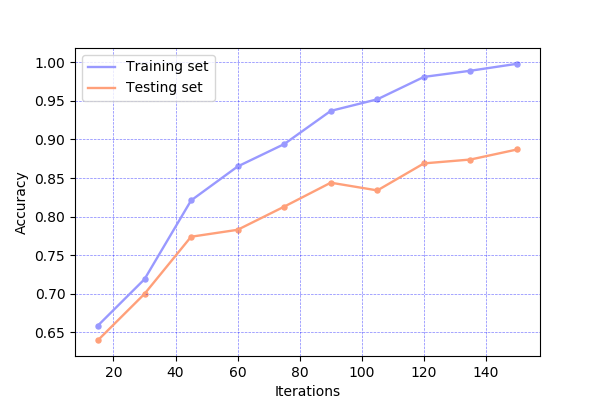
\includegraphics[width=0.45\linewidth]{img/svm_baseline_splice.png}
	}
	\subfigure[Satimage]{
		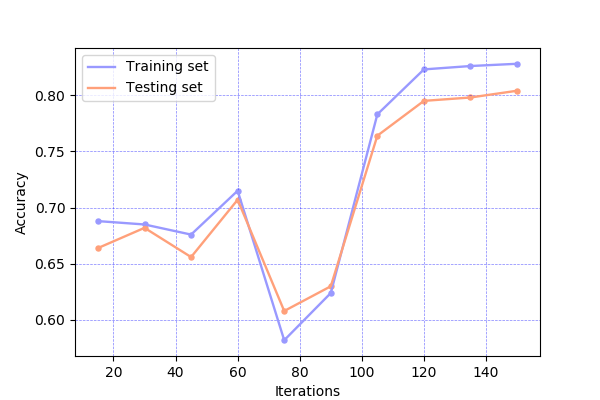
\includegraphics[width=0.45\linewidth]{img/svm_baseline_sat.png}
	}
	\caption{The baseline of SVM.}
	\label{fig:svm-baseline}
\end{figure}

\subsubsection{Kernel}

The ability of SVM might be constrainted when dealing with non-linear features, where kernel trick could resolve this issue. Nevertheless, a successful choice of kernel is still based on experience or luck. I apply several kernels to SVM and get the following results (Fig. \ref{fig:svm-kernel}).

\begin{figure}[H]
	\centering
	\subfigure[Splice-Training Set]{
		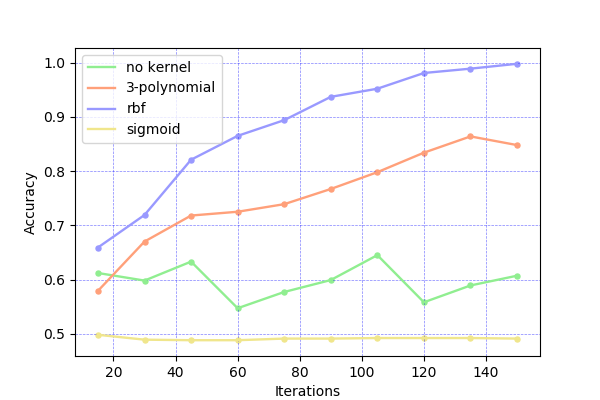
\includegraphics[width=0.45\linewidth]{img/svm_kernel_splice_tr.png}
	}
	\subfigure[Splice-Tetsing Set]{
		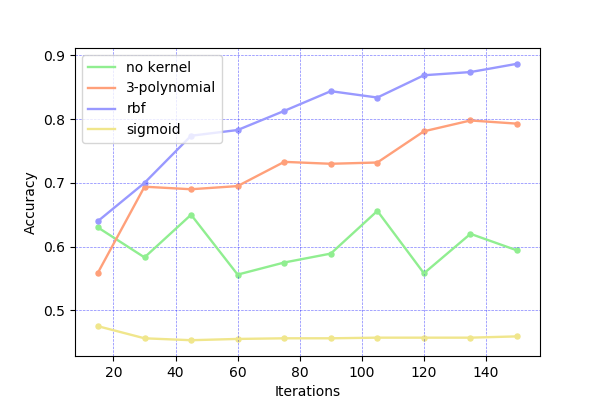
\includegraphics[width=0.45\linewidth]{img/svm_kernel_splice_t.png}
	}
	\subfigure[Satimage-Training Set]{
		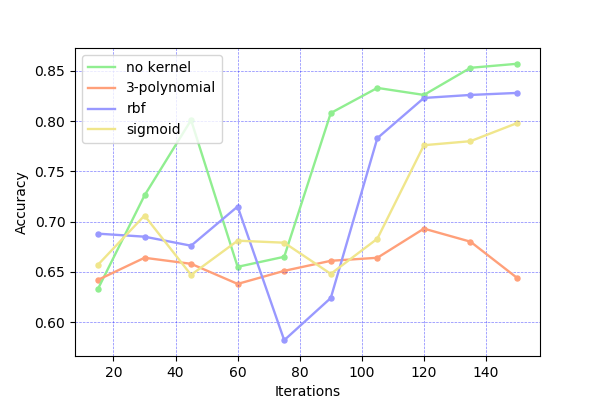
\includegraphics[width=0.45\linewidth]{img/svm_kernel_sat_tr.png}
	}
	\subfigure[Satimage-Testing Set]{
		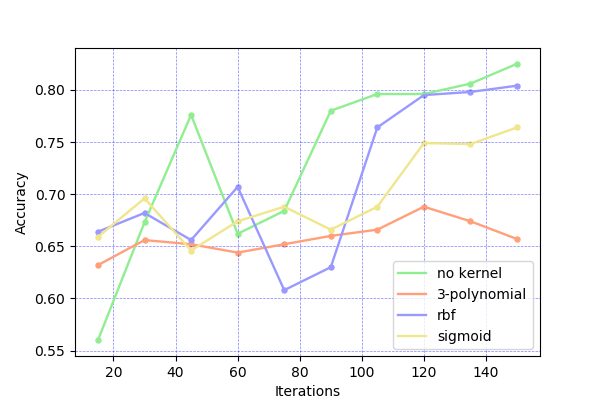
\includegraphics[width=0.45\linewidth]{img/svm_kernel_sat_t.png}
	}
	\caption{The performances of SVM under different kernels.}
	\label{fig:svm-kernel}
\end{figure}

\vspace{0.015\linewidth}
It is apparent that the effect of these kernels differ greatly. Rbf (Radial Basis Function) kernel is most suitable for \textit{splice} while no kernel function is the best choice for \textit{satimage}. 

\vspace{0.015\linewidth}
Additionally, the selection of specific parameters of a kernel would also affect the results. I test polynomial kernel with different degrees, the test error can refer to Tab. \ref{tab:kernel-poly}.

\vspace{0.015\linewidth}
\begin{table}[H]
	\renewcommand\arraystretch{1.35}
	\caption{The performances of polynomial kernel under different degrees}
	\label{tab:kernel-poly}
	\centering
	
	\begin{tabular}{c|c|c}
		\centering
		Degree & Test Error (Splice) & Test Error (Satimage) \\
		\hline
		
		2 & 0.786 & 0.635 \\
		3 & 0.857 & 0.666 \\
		4 & 0.865 & 0.505 \\
		5 & 0.871 & 0.554 \\
		6 & 0.880 & 0.488 \\
		7 & 0.874 & 0.512 \\
		8 & 0.864 & 0.477 \\
		9 & 0.867 & 0.528 \\
		10 & 0.851 & 0.403 \\
	\end{tabular}
\end{table}

The trend reflected in the above table is that higher degree can reduce training error, but lead to more test error in the meantime. Still, the performance would also drop a lot in both training set and testing set when the degree is too large. In short, this result proves the significance of choosing the complexity of model properly.

\vspace{0.01\linewidth}
\subsubsection{Penalty Parameter}

Although SVM would encounter difficulties on non-linear data, it can still handle slightly non-separable data via soft-margin technique: transforming the optimization object from 
\begin{equation*}
\dfrac{1}{2}w^Tw
\end{equation*}
into

\begin{equation*}
\dfrac{1}{2}w^Tw+C\sum\limits_{n=1}^{N}\xi_n,
\end{equation*}
where the penalty parameter $C$ is critical for classification performance. 

\vspace{0.01\linewidth}
I have tried the $C$ on different orders of magnitude, and the results can be found in Fig. \ref{fig:svm-penalty}.

\begin{figure}[H]
	\centering
	\subfigure[Splice]{
		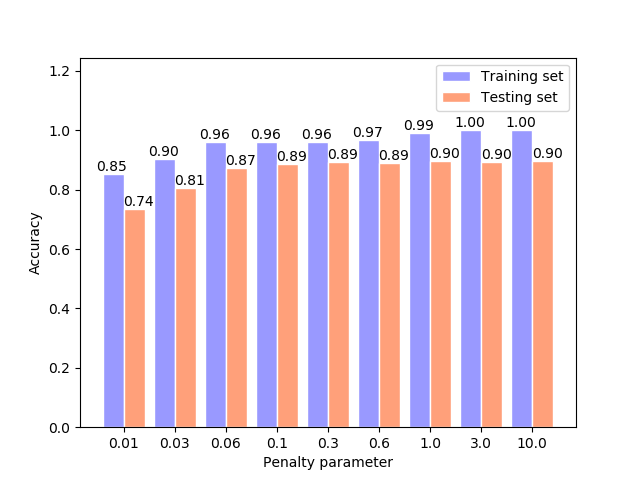
\includegraphics[width=0.48\linewidth]{img/svm_penalty_splice.png}
	}
	\subfigure[Satimage]{
		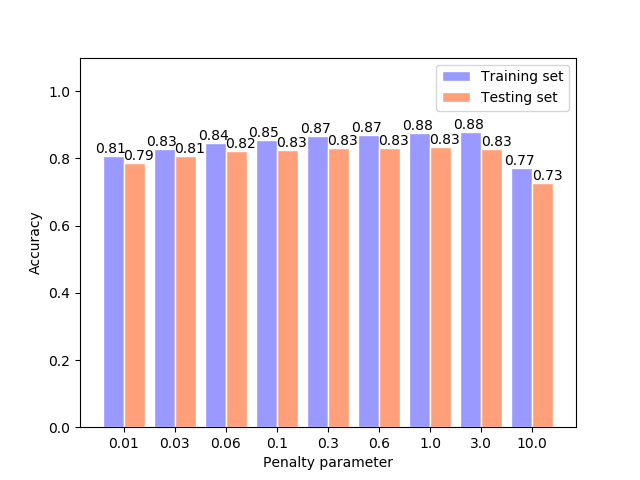
\includegraphics[width=0.48\linewidth]{img/svm_penalty_sat.png}
	}
	\caption{The performances of SVM under different penalty parameter $C$.}
	\label{fig:svm-penalty}
\end{figure}

According to the results, the introduction of $C$ is sometimes beneficial to the classification. More specifically, proper $C$ could improve the performance of SVM while excessive $C$ might produce additional errors.

\vspace{0.01\linewidth}
In general, the circumstances might vary a little bit according to the data, where $C$ should be determined by large scale of experiments.

\vspace{0.01\linewidth}
\subsubsection{Dimension of Features}
\label{sec:pca}

In some cases, the performance of a classification model might be reduced due to the redundant features of the dataset. Therefore, I test the performances of SVM under different variance radios of features. I implement this dimension reduction via PCA, corresponding results can refer to Fig. \ref{fig:svm-dim}.

\begin{figure}[H]
	\centering
	\subfigure[Splice-Training Set]{
		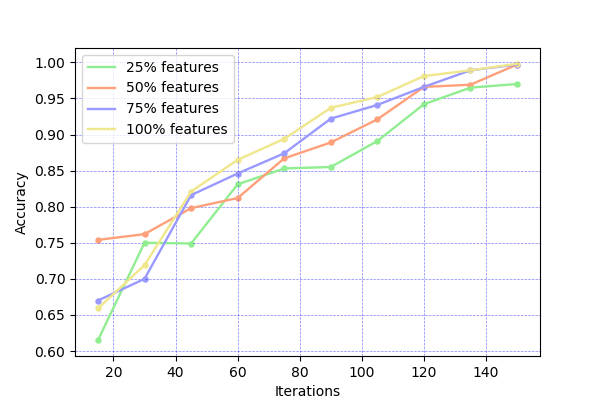
\includegraphics[width=0.45\linewidth]{img/svm_dim_splice_tr.png}
	}
	\subfigure[Splice-Tetsing Set]{
		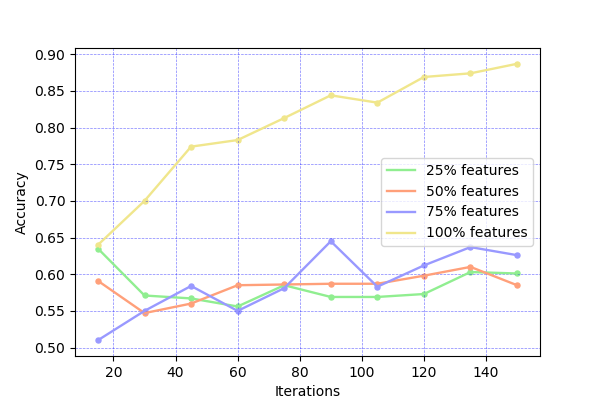
\includegraphics[width=0.45\linewidth]{img/svm_dim_splice_t.png}
	}
	\subfigure[Satimage-Training Set]{
		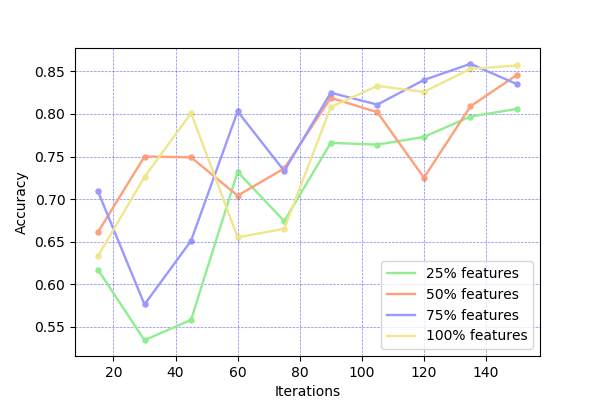
\includegraphics[width=0.45\linewidth]{img/svm_dim_sat_tr.png}
	}
	\subfigure[Satimage-Testing Set]{
		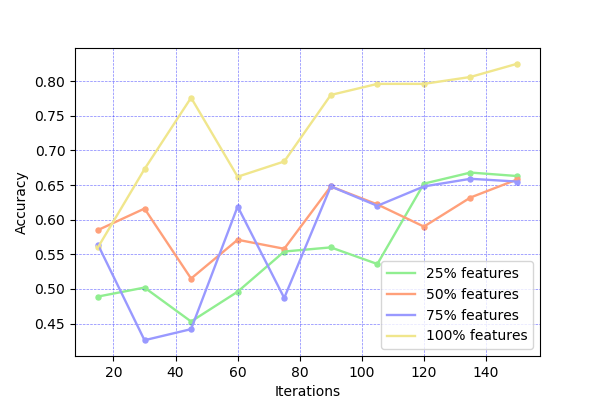
\includegraphics[width=0.45\linewidth]{img/svm_dim_sat_t.png}
	}
	\caption{The performances of SVM under different variance radios of features.}
	\label{fig:svm-dim}
\end{figure}

This result indicates both of \textit{splice} and \textit{satimage} have few redundant features, and less features lead to great performance reduction in testing set, namely affect the generalization ability.

\subsubsection{Summarization}

SVM is a powerful tool for classification, which can achieve satisfactory results in both binary and multi-class classification problems. Meanwhile, SVM could take advantages of many tricks (e.g. soft-margin, kernel) to extend its application scope and improve its performances. If SVM is applied to small scale problems with appropriate configurations, it would have a surprisingly performance.

\subsection{Neural Network}

In this section, I would also show the performances of MLP in \textit{splice} and \textit{satimage} under different configurations (e.g. optimization algorithms, network architectures). In the meantime, I would also analyze each result concisely. Note that MLP and neural network here are the same meaning. CNN might achieve better performances, but my computing resources can hardly afford it.

\vspace{0.01\linewidth}
Same as Sec. \ref{sec:svm}, I conduct the following experiments based on default parameters in \textit{sklearn}. Some important parameters are shown in Tab. \ref{tab:default-para-mlp} and the baseline model can refer to Fig. \ref{fig:mlp-baseline}.

\begin{table}[H]
	\renewcommand\arraystretch{1.35}
	\caption{Some important default parameters of MLP experiments}
	\label{tab:default-para-mlp}
	\centering
	
	\begin{tabular}{c|c|c}
		\centering
		Name & Meaning & Value \\
		\hline
		\hline
		
		hidden\_layer\_sizes & the size of hidden layers & (100,) \\
		activation & activation function for the hidden layer & relu \\
		solver & the solver for weight optimization & adam \\
		alpha & L2 penalty (regularization term) parameter & 0.0001 \\
		batch\_size & size of minibatches for stochastic optimizers & min(200, n\_samples) \\
		learning\_rate\_init & the initial learning rate used & 0.001 \\
		power\_t & the exponent for inverse scaling learning rate & 0.5 \\
		tol & tolerance for the optimization & 1e-4 \\
		
	\end{tabular}
\end{table}

\begin{figure}[H]
	\centering
	\subfigure[Splice]{
		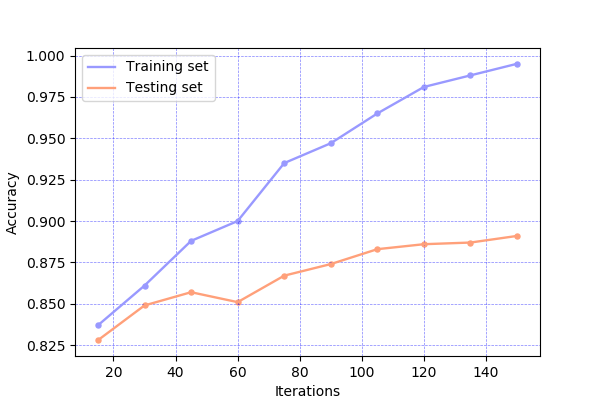
\includegraphics[width=0.45\linewidth]{img/mlp_baseline_splice.png}
	}
	\subfigure[Satimage]{
		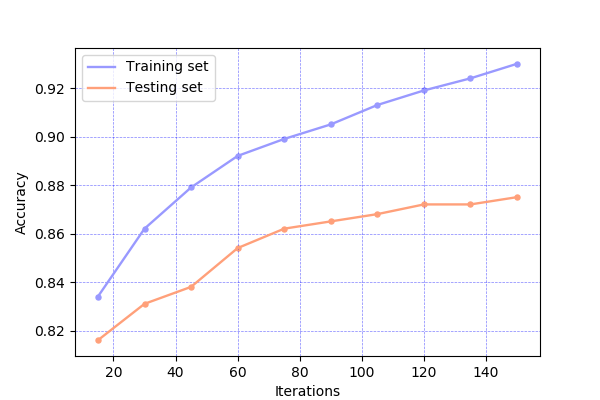
\includegraphics[width=0.45\linewidth]{img/mlp_baseline_sat.png}
	}
	\caption{The baseline of MLP.}
	\label{fig:mlp-baseline}
\end{figure}

\subsubsection{Optimization Algorithm}
\label{sec:optim}

Optimization algorithms refer to a series algorithms used to update parameters of neural network (e.g. sgd, adam \cite{adam}). The optimal directions and the effects of these algorithms are quite different, Fig. \ref{fig:example} is a visual illustration.

\begin{figure}[H]
	\centering
	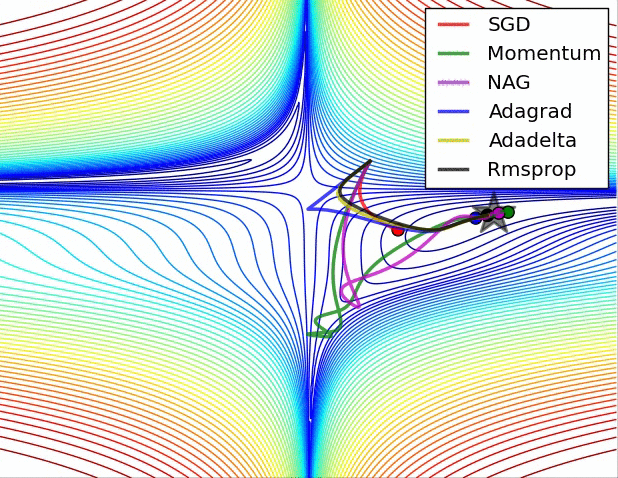
\includegraphics[width=0.45\linewidth]{img/optim_example.png}
	\caption{The visual illustration of optimization algorithms \cite{optim_example}.}
	\label{fig:example}
\end{figure}

Since the performance of MLP is greatly influenced by the optimization algorithms, I tend to investigate it in detail. I test the effects of three typical algorithms: \textbf{lbfgs}, \textbf{sgd} and \textbf{adam}. The corresponding training processes are shown in Fig. \ref{fig:mlp-optimizer}.

\begin{figure}[H]
	\centering
	\subfigure[Splice-Training Set]{
		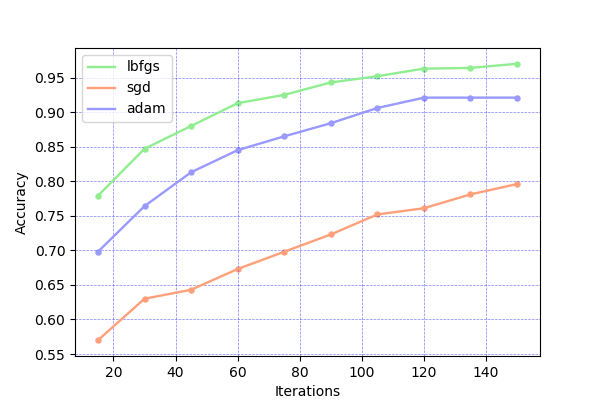
\includegraphics[width=0.45\linewidth]{img/mlp_optimizer_splice_tr.png}
	}
	\subfigure[Splice-Tetsing Set]{
		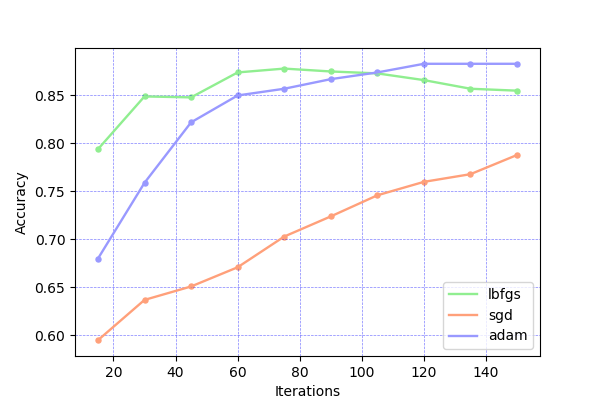
\includegraphics[width=0.45\linewidth]{img/mlp_optimizer_splice_t.png}
	}
	\subfigure[Satimage-Training Set]{
		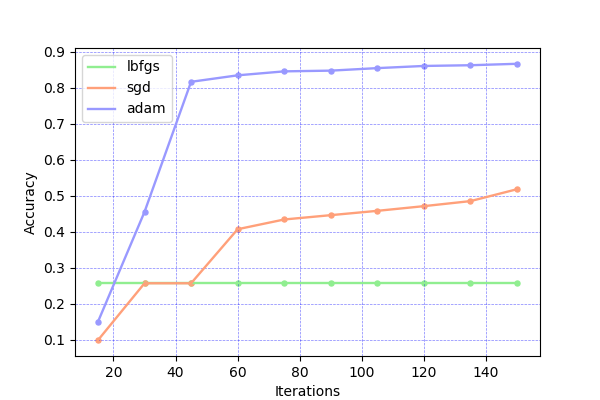
\includegraphics[width=0.45\linewidth]{img/mlp_optimizer_sat_tr.png}
	}
	\subfigure[Satimage-Testing Set]{
		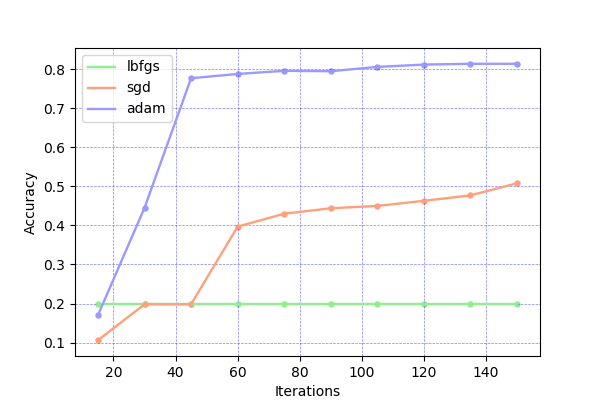
\includegraphics[width=0.45\linewidth]{img/mlp_optimizer_sat_t.png}
	}
	\caption{The performances of MLP under different optimization algorithms.}
	\label{fig:mlp-optimizer}
\end{figure}

The results in two datasets are consistent with the theoretical analysis: the effect of optimization algorithms differ awfully. It seems that \textit{adam} achieves the best performance in both datasets (though \textit{lbfgs} has lower training error, it might encounter overfitting in \textit{splice}). In \textit{satimage}, the rest two algorithms have poor performance, \textit{lbfgs} even falls into a local minimum at the beginning of training.

\vspace{0.01\linewidth}
In brief, \textit{adam} algorithm could achieve satisfactory results in most cases, the optimization effect of \textit{sgd} is weaker and \textit{lbfgs} might be instable.

\subsubsection{Activation Function}

Activation function is an indispensable component of MLP. It extends the scope that MLP can represent by introducing non-linear factors into MLP. I compare the effects of 3 commonly used activation functions (\textbf{relu} \cite{relu}, \textbf{sigmoid} and \textbf{tanh}) on the two datasets (Fig. \ref{fig:mlp-activation}).

\begin{figure}[H]
	\centering
	\subfigure[Splice-Training Set]{
		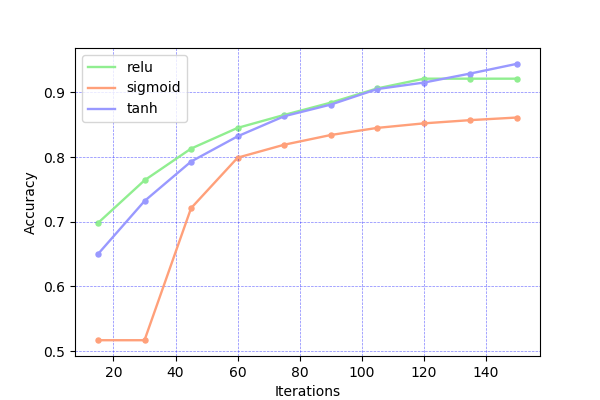
\includegraphics[width=0.43\linewidth]{img/mlp_activation_splice_tr.png}
	}
	\subfigure[Splice-Tetsing Set]{
		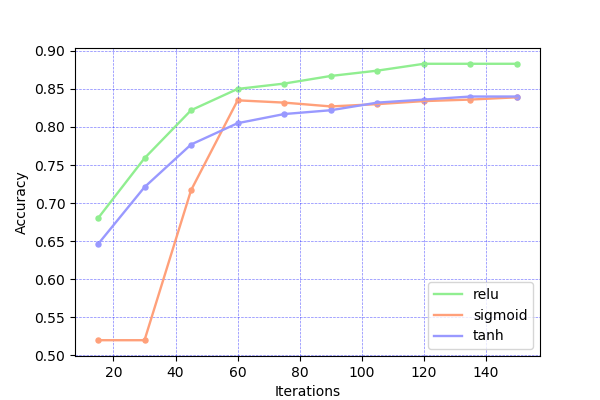
\includegraphics[width=0.43\linewidth]{img/mlp_activation_splice_t.png}
	}
	\subfigure[Satimage-Training Set]{
		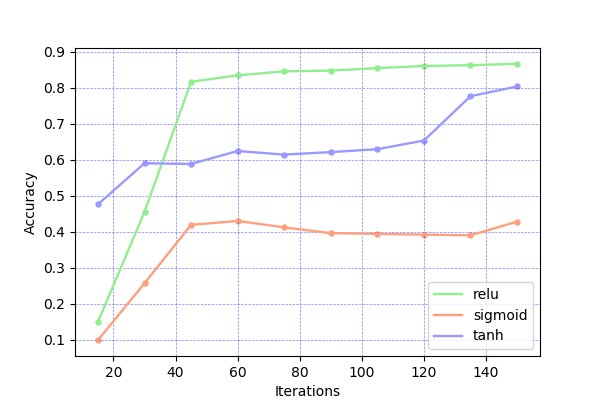
\includegraphics[width=0.43\linewidth]{img/mlp_activation_sat_tr.png}
	}
	\subfigure[Satimage-Testing Set]{
		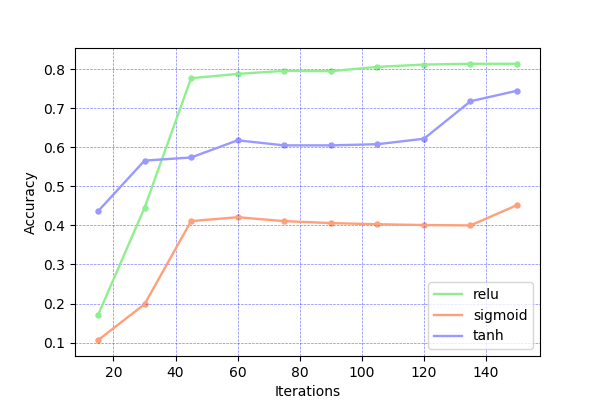
\includegraphics[width=0.43\linewidth]{img/mlp_activation_sat_t.png}
	}
	\caption{The performances of MLP under different activation functions.}
	\label{fig:mlp-activation}
\end{figure}

Similar to Sec. \ref{sec:optim}, the effects of different activation function are widely divergent, especially on \textit{satimage}. In most cases, \textit{relu} is undoubtedly the best choice. \textit{sigmoid} and \textit{tanh} could be applied to simple problems, their effects would be greatly reduced when confronted with complex problems.

\subsubsection{Learning Rate}

In training process, learning rate controls the speed of parameters updating. Researchers often pours quantities of time into adjusting learning rate due to its large effect to training results. I investigate the classification results on several orders of magnitude of learning rate (Fig. \ref{fig:mlp-lr}).

\vspace{-0.01\linewidth}
\begin{figure}[H]
	\centering
	\subfigure[Splice]{
		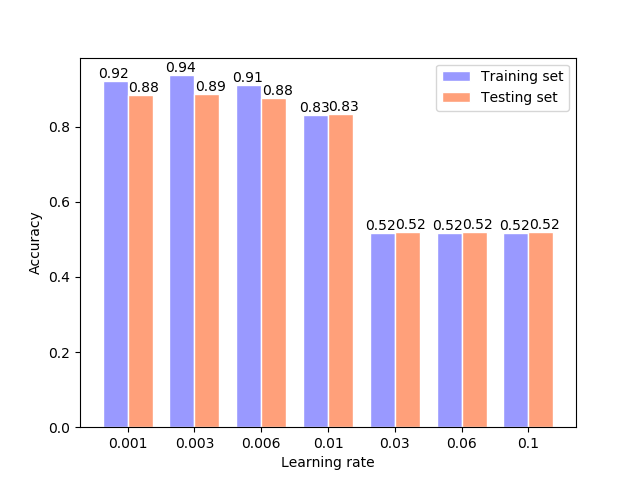
\includegraphics[width=0.43\linewidth]{img/mlp_lr_splice.png}
	}
	\subfigure[Satimage]{
		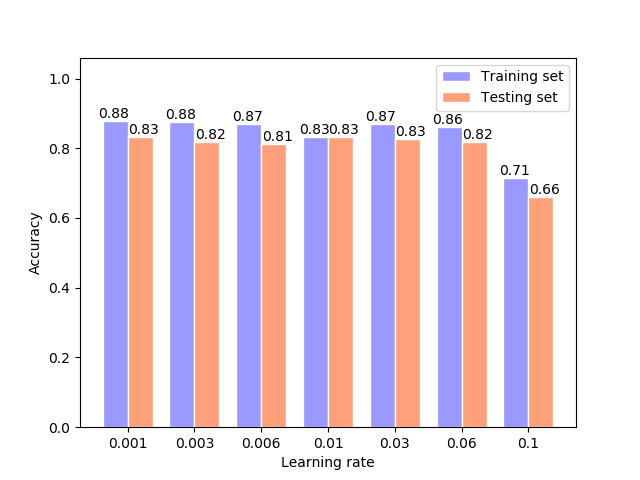
\includegraphics[width=0.43\linewidth]{img/mlp_lr_sat.png}
	}
	\caption{The performances of MLP under different learning rate.}
	\label{fig:mlp-lr}
\end{figure}

According to above results, learning rates of 0.003 and 0.001 could provide the best performances for MLP on \textit{splice} and \textit{satimage} respectively. Unfortunately, even the best results in Fig. \ref{fig:mlp-lr} have no improvement compared with baseline (Fig. \ref{fig:mlp-baseline}), this also illustrates the difficulty on choosing a appropriate learning rate.

\subsubsection{Network Architecture}

In addition to the above configuration factors, the network architecture of MLP also contributes a lot to final results. There are two simple changes to the network architecture: deepening the network and increasing the number of neurons of each layer. I have tried several architectures based on these two changes (Fig. \ref{fig:mlp-archi}).

\begin{figure}[H]
	\centering
	\subfigure[Splice-Training Set]{
		\label{fig:mlp-archi-a}
		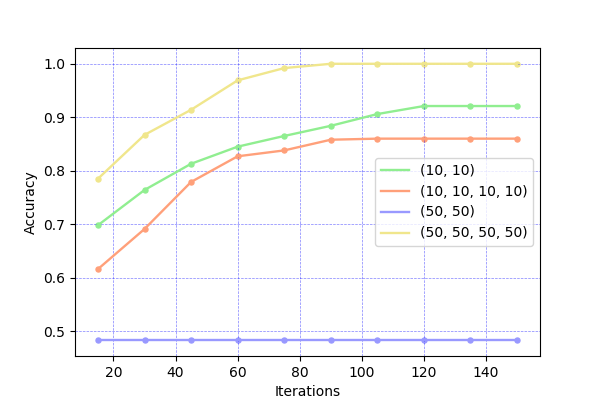
\includegraphics[width=0.48\linewidth]{img/mlp_archi_splice_tr.png}
	}
	\subfigure[Splice-Tetsing Set]{
		\label{fig:mlp-archi-b}
		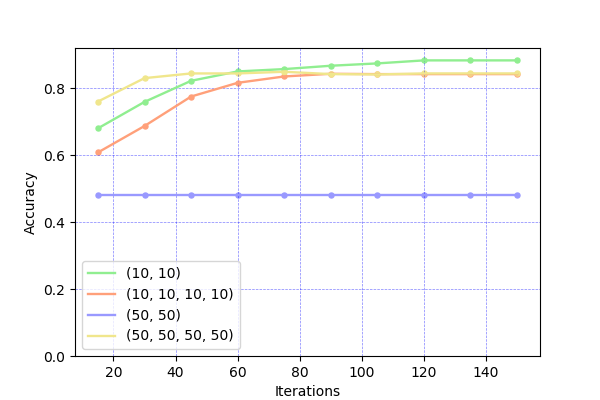
\includegraphics[width=0.48\linewidth]{img/mlp_archi_splice_t.png}
	}
	\subfigure[Satimage-Training Set]{
		\label{fig:mlp-archi-c}
		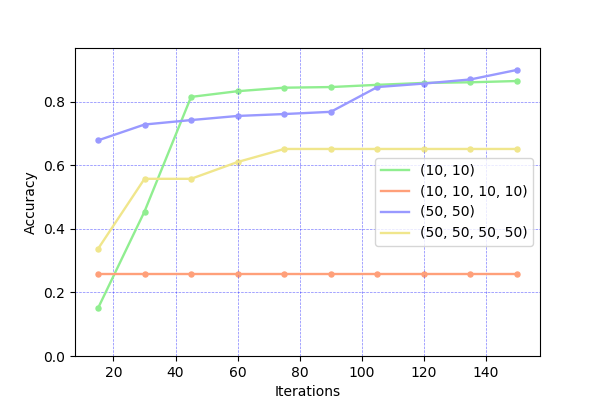
\includegraphics[width=0.48\linewidth]{img/mlp_archi_sat_tr.png}
	}
	\subfigure[Satimage-Testing Set]{
		\label{fig:mlp-archi-d}
		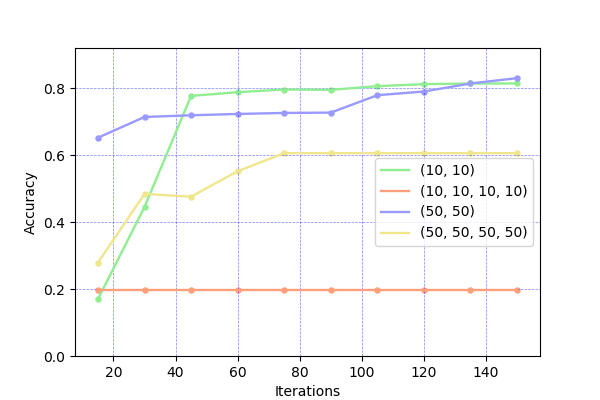
\includegraphics[width=0.48\linewidth]{img/mlp_archi_sat_t.png}
	}
	\caption{The performances of MLP under different network architectures (the numbers in brackets indicate the number of neurons in each layer).}
	\label{fig:mlp-archi}
\end{figure}

For a certain dataset, appropriate architectures would bring about good performances, like red and yellow lines in Fig. \ref{fig:mlp-archi-b} and yellow line in Fig. \ref{fig:mlp-archi-d}. Otherwise, unsuitable architectures might crash the whole training process (blue line in Fig. \ref{fig:mlp-archi-b} and red line in Fig. \ref{fig:mlp-archi-d}).

\subsubsection{Dimension of Features}

Similar to Sec. \ref{sec:pca}, I also fit my MLP model under different variance radios of features (Fig. \ref{fig:mlp-dim}).

\begin{figure}[H]
	\centering
	\subfigure[Splice-Training Set]{
		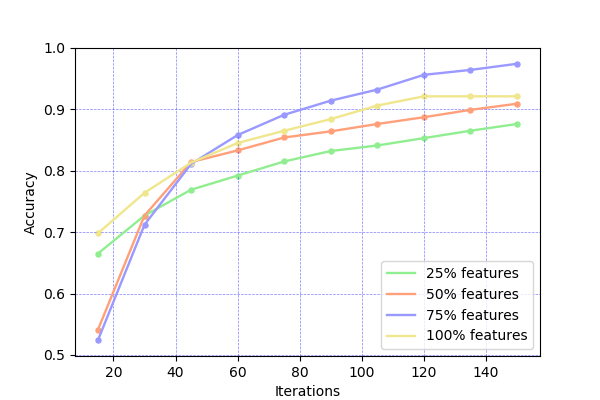
\includegraphics[width=0.48\linewidth]{img/mlp_dim_splice_tr.png}
	}
	\subfigure[Splice-Tetsing Set]{
		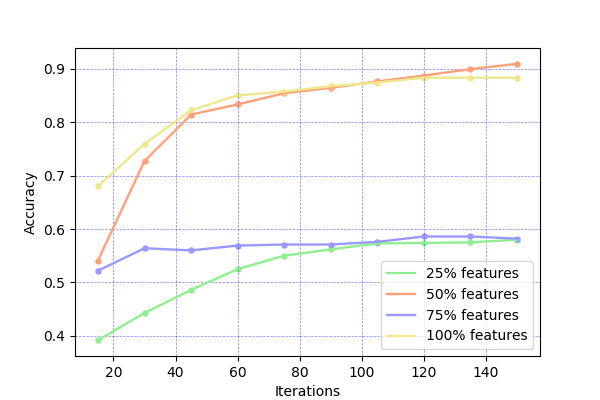
\includegraphics[width=0.48\linewidth]{img/mlp_dim_splice_t.png}
	}
	\subfigure[Satimage-Training Set]{
		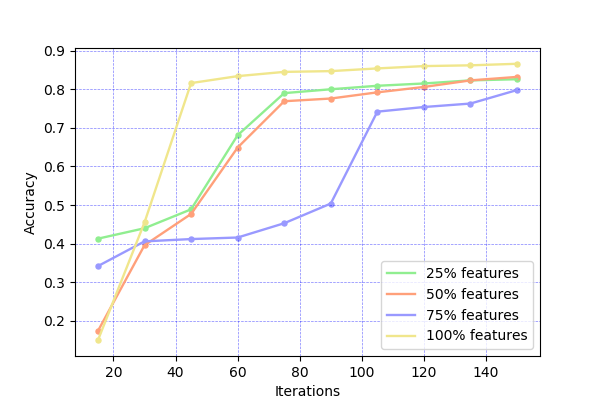
\includegraphics[width=0.48\linewidth]{img/mlp_dim_sat_tr.png}
	}
	\subfigure[Satimage-Testing Set]{
		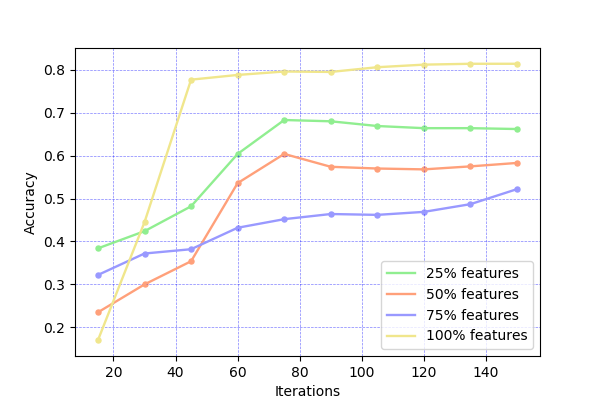
\includegraphics[width=0.48\linewidth]{img/mlp_dim_sat_t.png}
	}
	\caption{The performances of MLP under different variance radios of features.}
	\label{fig:mlp-dim}
\end{figure}

The above result has the same trend as that in Fig. \ref{fig:svm-dim}, which is reasonable due to the same datasets are used.

\subsubsection{Summarization}
\label{sec:sum-mlp}

MLP is a common way for a variety of problems. It owns a broader representation ability and stability compared with SVM and the baselines (Fig. \ref{fig:svm-baseline} and Fig. \ref{fig:mlp-baseline}) also prove this.

\vspace{0.01\linewidth}
Still, an available MLP model often takes much time to finetune, even a small change on any one component might make a great difference.

\section{Comparison Between SVM and Deep Learning Algorithm Benchmarks}

In this section, I would apply SVM on CIFAR-10 dataset \cite{cifar-10} and compare the results to corresponding deep learning algorithm benchmarks. These results were obtained with convolutional neural networks or some other fancy network architectures.

\subsection{Baseline of SVM}
\vspace{0.01\linewidth}

I first fit SVM with default parameters of \textit{sklearn} on CIFAR-10 and get a terrible result: 88\% training error and 90\% test error with 10000 iterations, taking about 20 minutes on a INTEL I5-5200U CPU. I infer that such result might be out of the high dimension of features and large scale of samples. Then I start to adjust the SVM model to improve its performance.

\subsection{Finetune}
\label{sec:finetune}

In this section, I would show the process of finetuning my SVM model. Due to the limited computing resources, I can hardly conduct perfectly comprehensive experiments. I tend to focus on the points I think are pivotal. Note that I only need to observe the trend here, so I just use the original data to finetune parameters in 1000 iterations.

\paragraph{1. Kernel}

\vspace{0.01\linewidth}
Since the performance of SVM on CIFAR-10 is pretty poor, I think it is difficult to improving this just by adjusting some numerical parameters. Therefore, I start with picking out the most appropriate kernel.

\vspace{0.01\linewidth}
I have tried 3 kinds of kernels on each batch of CIFAR-10 with 1000 iterations and default parameters of \textit{sklearn}. The results can refer to Tab. \ref{tab:bonus-kernel}.

\begin{table}[H]
	\renewcommand\arraystretch{1.5}
	\caption{The performances of different kernels on CIFAR-10}
	\label{tab:bonus-kernel}
	\centering
	
	\begin{tabular}{c|c|c|c|c|c|c}
		\centering
		 & Batch 1 & Batch 2 & Batch 3 & Batch 4 & Batch 5 & Whole data \\
		\hline
		\hline
		
		Rbf (training error) & 0.193 & 0.192 & 0.196 & 0.192 & 0.198 &  0.123 \\
		Rbf (test error) & 0.105 & 0.103 & 0.105 & 0.105 & 0.105 & 0.105 \\
		Polynomial (training error) & 0.223 & 0.236 & 0.245 & 0.248 & 0.244 & 0.170 \\
		Polynomial (test error) & 0.209 & 0.218 & 0.213 & 0.229 & 0.228 & 0.172 \\
		Sigmoid (training error) & 0.098 & 0.098 & 0.103 & 0.098 & 0.102 & 0.100 \\
		Sigmoid (test error) & 0.100 & 0.100 & 0.100 & 0.100 & 0.100 & 0.100 \\
		Linear kernel (training error) & 0.234 & 0.201 & 0.254 & 0.249 & 0.209 & 0.191 \\
		Linear kernel (test error) & 0.218 & 0.184 & 0.240 & 0.223 & 0.186 & 0.180 \\
	\end{tabular}
\end{table}

As is shown in the above table, linear kernel achieves best performance, polynomial kernel is the next one and sigmoid kernel owns the worst performance. Nevertheless, the performances of other kernels are still possible to exceed that of linear kernel by modifying corresponding parameters.

\paragraph{2. Parameters of Rbf Kernel}

Basically, rbf kernel ($K(x_i, x_j)=exp(-\gamma\|x_i-x_j\|^2), \gamma>0$) is the most commonly applied kernel function, linear kernel is just a special case of rbf kernel and sigmoid kernel tend to be similar with rbf kernel under some special parameters. Compared with poly kernel, rbf kernel has less parameters to train and would reduce the difficulty of calculating.

\vspace{0.015\linewidth}
In consideration of the above factors, I decide to adjust the $\gamma$ of rbf kernel to obtain a better performance (Tab. \ref{tab:rbf-para}), the default value is the $1/numberOfFeatures$, namely $1/3072=0.0003$.\footnote{The parameters adjustments for other kernels can refer to Appendix \ref{apd:para-adj}.}

\begin{table}[H]
	\renewcommand\arraystretch{1.35}
	\caption{The performances of different kernels on CIFAR-10 (Considering the limited computing resources, I treat the performance on batch 1 as a representation of that in whole data)}
	\label{tab:rbf-para}
	\centering
	
	\begin{tabular}{c|c|c}
		\centering
		The value of $\gamma$ & Training error on batch 1 & Test error on batch 1 \\
		\hline
		\hline
		
		$3 \times 10^{-7}$ & 0.411 & 0.318 \\
		$3 \times 10^{-7}$ & 0.464 & 0.330 \\
		$6 \times 10^{-7}$ & 0.470 & 0.304 \\
		$1 \times 10^{-6}$ & 0.466 & 0.282 \\
		$3 \times 10^{-6}$ & 0.423 & 0.229 \\
		$6 \times 10^{-6}$ & 0.404 & 0.233 \\
		$1 \times 10^{-5}$ & 0.344 & 0.242 \\
		$3 \times 10^{-5}$ & 0.320 & 0.239 \\
		$6 \times 10^{-5}$ & 0.319 & 0.238 \\
		$1 \times 10^{-4}$ & 0.309 & 0.227 \\
		$3 \times 10^{-4}$ & 0.193 & 0.105 \\
		$1 \times 10^{-3}$ & 0.188 & 0.100 \\
		$3 \times 10^{-3}$ & 0.188 & 0.100 \\
		$6 \times 10^{-3}$ & 0.188 & 0.100 \\
		$1 \times 10^{-2}$ & 0.188 & 0.100 \\
	\end{tabular}
\end{table}

\paragraph{3. Penalty Parameter}

Ultimately, I focus on finetuning penalty parameter $C$. $C$ represents the tolerance for error, inappropriate $C$ would reduce the generalization ability of SVM model. I adjust $C$ based on the best result above (results can be found in Fig. \ref{fig:penalty-para}).

\begin{figure}[H]
	\centering
	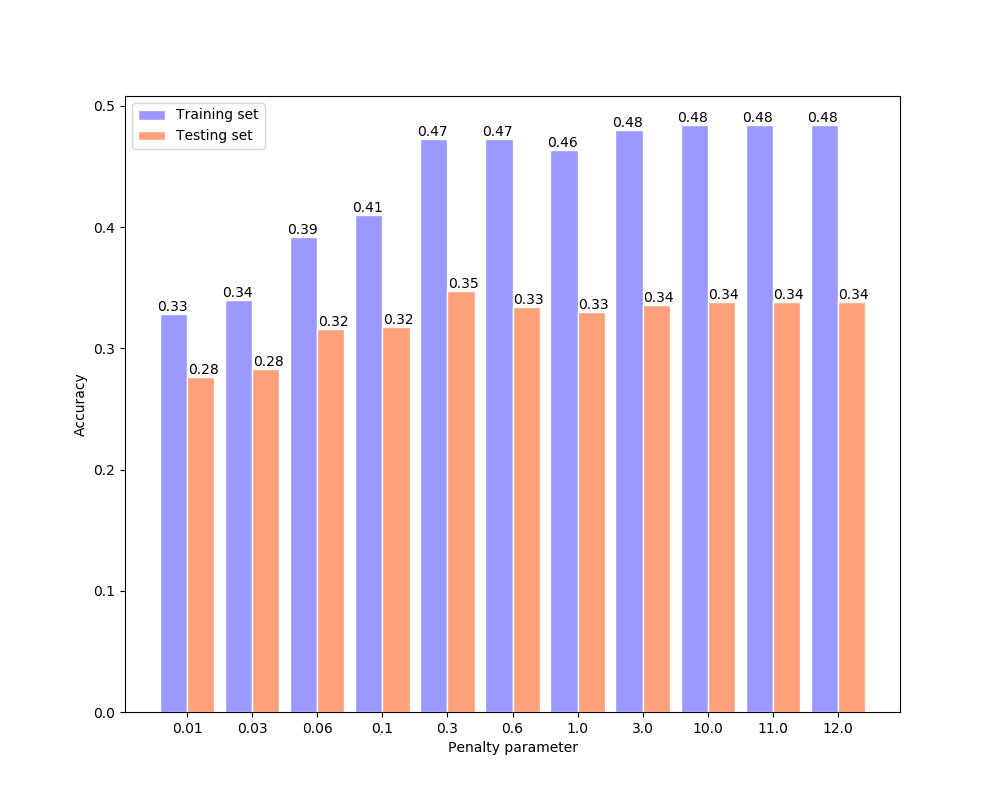
\includegraphics[width=0.65\linewidth]{img/para_penalty.png}
	\caption{The performances of SVM model under different penalty parameters.}
	\label{fig:penalty-para}
\end{figure}

Based on the above results, I infer that the most appropriate $C$ for SVM on CIFAR-10 might near 10.0. Further explorations narrow this scope (Tab \ref{tab:penalty-para}).

\vspace{-0.005\linewidth}
\begin{table}[H]
	\renewcommand\arraystretch{1.2}
	\caption{The performances of different penalty parameters $C$ on CIFAR-10}
	\label{tab:penalty-para}
	\centering
	
	\begin{tabular}{c|c|c}
		\centering
		The value of $C$ & Training error on batch 1 & Test error on batch 1 \\
		\hline
		\hline
		
		7.5 & 0.484 & 0.338 \\
		8.0 & 0.484 & 0.338 \\
		8.5 & 0.484 & 0.338 \\
		9.0 & 0.484 & 0.338 \\
		9.5 & 0.484 & 0.338 \\
		10.0 & 0.484 & 0.338 \\
		10.5 & 0.484 & 0.338 \\
	\end{tabular}
\end{table}

\vspace{-0.005\linewidth}
Since the values of $C$ in the above table correspond to the same performance, I just select $C$ as 10.0 for my SVM model.

\vspace{-0.015\linewidth}
\subsection{Final Result}
\label{sec:final_res}

\vspace{-0.01\linewidth}
So far, I have got relatively appropriate parameters of SVM model, then I compare it with some deep learning algorithm benchmarks \cite{bench} (Tab. \ref{tab:res}). To give full play to the performance of SVM, I also employ some preprocessing methods. Note that I remove the limitation of the number of training iterations and train SVM model until it converges.

\vspace{-0.015\linewidth}
\begin{table}[H]
	\renewcommand\arraystretch{1.25}
	\caption{The comparisons between SVM (without limitation of the number of iterations) and deep learning algorithm benchmarks, some results might be missing due to the massive time consumption}
	\label{tab:res}
	\centering
	
	\begin{tabular}{c|c}
		\centering
		Model & Test error on CIFAR-10 (\& training time) \\
		\hline
		\hline
		
		SVM & ??\% \quad more than 10 hours \\
		SVM (standardization) & 77.69\% \quad \\
		SVM (max-min normalization) & 78.25\% \quad \\
		SVM (pca 90\% variance radio) & 88.60\% \quad 21 min \\
		SVM (pca 80\% variance radio) & 89.00\% \quad 5 min \\
		SVM (standardization and pca 90\% variance) & 93.97\% \quad 16 min\\
%		SVM & 74.05\% \\
%		SVM (standardization) & 77.69\% \\
%		SVM (max-min normalization) & 78.25\% \\
%		SVM (pca 90\% variance) & 88.60\% \\
%		SVM (pca 80\% variance) & 89.00\% \\
%		SVM (standardization and pca 90\% variance) & 93.97\% \\
		\hline
		Fractional Max-Pooling \cite{bench2} & 3.47\% \\
		Spatially-sparse CNN \cite{bench10} & 6.28\% \\
		5-layers MLP & 6.37\% \\
		Batch-normalized maxout NIN \cite{bench3} & 6.75\% \\
		NIN \cite{bench4} & 8.20\% \\
		Maxout Networks \cite{bench5} & 8.80\% \\
		Cuda-convnet \cite{bench1} (with data augmentation) & 11.00\% \\
		Multi-Column DNN \cite{bench6} & 11.21\% \\
		ReNet \cite{bench9} & 12.35\% \\
		Cuda-convnet (without data augmentation) & 13.00\% \\
		Convolutional Kernel Networks \cite{bench7} & 17.82\% \\
		PCANet \cite{bench8} & 21.33\% \\
	\end{tabular}
\end{table}

The results indicate that the performances of SVM on CIFAR-10 are greatly inferior to deep learning algorithms. Besides, some common data preprocessing methods are of no avail for SVM under this circumstance.

\subsection{Strengths and Weaknesses of SVM on Big Datasets}

According to the results in Sec. \ref{sec:finetune} and Sec. \ref{sec:final_res}, SVM performs poorly on a big dataset CIFAR-10. Note that the so-called 'big dataset' here refer to those datasets with more than 10,000 samples or 1,000 features. In combination with the theoretical and experimental results, I think the weaknesses of SVM on big datasets consist of the following aspects:

\begin{enumerate}
	\item Basically, the aim of SVM is to find hyper-planes. When the distribution of data is not comprehensive enough, most data might be beneficial to adjust the planes. Once the data has enough coverage, most data would have no influence to planes, and some noise data might even be considered as support vectors. Then the model tends to contain more support vectors and encounter over-fitting problem;
	
	\item The support vectors are solved via quadratic programming, which would consume quantities of memories and time under large scale of samples. Suppose the number of samples and features are $n$ and $m$ respectively, the complexity of SVM is $O(mn^2)$ when using kernel tricks (e.g. rbf kernel);
	
	\item The classical SVM mainly deals with binary classification problems, while most big datasets are constucted for multi-class classification. Under such circumstances, the most common solution is to combine multiple SVM models (e.g. one-vs-one, one-vs-rest). Still, the performance of SVM on multi-class classification is inferior to binary classification problems;
	
	\item A common weakness of machine learning algorithms on big datasets is the tremendous cost for parameters adjustment, SVM is no exception, which has been discussed detailedly in Sec. \ref{sec:svm}. Additionally, SVM also suffers from unstable problems sometimes.
\end{enumerate}

Although SVM has the above weaknesses on big datasets, it also owns some unique strengths:

\begin{enumerate}
	\item SVM constructs its optimal hyper-plane based on structural risk minimization theory, which could be represented as a convex optimization problem. Since such problems have been thoroughly solved, SVM would be more likely to obtain global optimum solution, while most popular methods like MLP only achieve local minimum in most cases;
	
	\item Since the optimization objective of SVM could be solved by classical algorithms, SVM owns faster convergence velocity than neural network and some other machine learning algorithms. That is, SVM would converge with less iterations on big datasets, despite of the enormous time consumption for each iteration.
\end{enumerate}

In conclusion, SVM is a flexible and high-performanced model on small or medium datasets, where SVM can achieve similar performances to neural network (e.g. MLP). However, SVM is inappropriate for big datasets, where its weaknesses, especially the time cinsumption, might conceal its strengths in most cases. Still, methods to make up for the weaknesses are being constantly developed (e.g. parallelization to optimize time consumption).

\newpage
\begin{appendix}
\section{Appendix}

\subsection{Details of Datasets in Experiments}
\label{apd:dataset}

\subsubsection{Splice \cite{splice}}

Basically, according to the biological knowledge, splice junctions are points on a DNA sequence at which `superfluous' DNA is removed during the process of protein creation in higher organisms.

\vspace{0.01\linewidth}
Splice dataset aims to recognize two classes of splice junctions, given a DNA sequence, the boundaries between exons (the parts of the DNA sequence retained after splicing) and introns (the parts of the DNA sequence that are spliced out).

\subsubsection{Satimage \cite{satimage}}

Satimage dataset is also called \textbf{satalog} dataset. It contains multi-spectral values of pixels in 3 $\times$ 3 neighbourhoods in satellite images, and the classification associated with the central pixel in each neighbourhood.

\vspace{0.01\linewidth}
As a classification dataset, the aim of satimage is to predict the classification, given the multi-spectral values. In the sample database, the class of a pixel is coded as a number.

\subsubsection{CIFAR-10 \cite{cifar-10}}

The CIFAR-10 dataset is labeled subsets of the 80 million tiny images dataset, collected by Alex Krizhevsky, Vinod Nair, and Geoffrey Hinton. CIFAR-10 consists of 60000 $32 \times 32$ colour images (50000 for training (divided into 5 batches), 10000 for test) in 10 classes, with 6000 images per class.

\vspace{0.01\linewidth}
Note that the classes of CIFAR-10 are completely mutually exclusive and there is no overlap between two classes (e.g. automobiles and trucks).

\subsection{The Parameters Adjustments of Kernels.}
\label{apd:para-adj}

\begin{figure}[H]
	\centering
	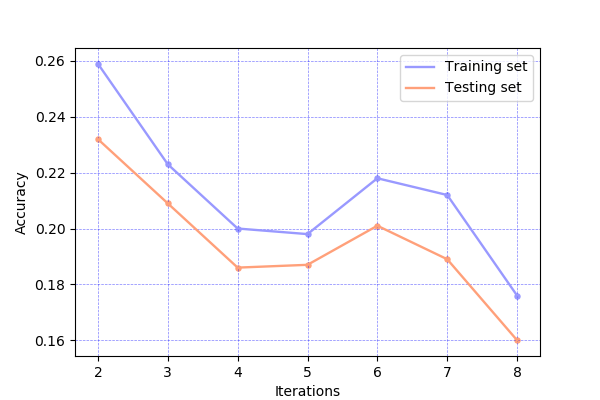
\includegraphics[width=0.7\linewidth]{img/svm_poly_para.png}
	\caption{The performances of polynomial kernel under different degrees.}
	\label{fig:para-adj-poly}
\end{figure}


\end{appendix}

\bibliographystyle{ieeetr}
\bibliography{bio}

\end{document}